\section{Ćwiczenia 3: 9-III-2017}
\subsection{Zadania domowe A}
\paragraph{A1} Chcemy wysłać dużą partię towarów, pakując je w paczki. Wprawdzie do jednej paczki zmieściłyby się wszystkie towary, ale ze względów bezpieczeństwa nie każdy może podróżować z każdym w jednej paczce. Wiemy, jakie towary możemy zapakować razem, a jakie nie. Naszym celem jest wyznaczyć ile najmniej paczek potrzeba do transportu. Zinterpertuj problem w języku grafów.  Jaki parametr grafowy nas   interesuje?   

\textbf{Odpowiedź:} 
\begin{itemize}
\item wierzchołek $\rightarrow $  towar 
\item krawędź $\rightarrow $ towar nie może być zapakowany z innym towarem
\item kolor $\rightarrow $ paczka, w której nie ma wierzchołków połączonych krawędzią
\item minimalna liczba paczek $\rightarrow $ liczba kolorów
\end{itemize}

\paragraph{A2} Narysuj graf, który nie zawiera $K_4$, ale
\begin{enumerate}[label=(\alph*)]
\item zawiera $K_4$ jako minor,
\item zawiera topologiczną kopię $K_4$.
\end{enumerate}
\textbf{Odpowiedź:} \\
\begin{minipage}{.32\textwidth}
\begin{figure}[H]
\centering
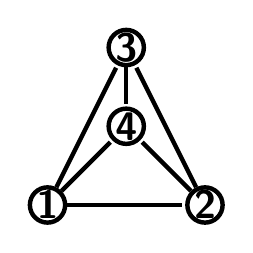
\begin{tikzpicture}[shorten >=1pt, auto, node distance=3cm, ultra thick,main node/.style={circle,draw,minimum size=.4cm,inner sep=0pt]}]%fill=black,
\begin{scope}[every node/.style={font=\sffamily\Large\bfseries}]
\node[main node] (v1) at (0,0) {1};
\node[main node] (v2) at (2,0) {2};
\node[main node] (v3) at (1,2) {3};
\node[main node] (v4) at (1,1) {4};
%\node[main node] (v) at (,) {};
\end{scope}
\begin{scope}
\draw  (v1) edge node{} (v2);
\draw  (v1) edge node{} (v3);
\draw  (v1) edge node{} (v4);
\draw  (v2) edge node{} (v3);
\draw  (v2) edge node{} (v4);
\draw  (v3) edge node{} (v4);
%\draw  (v) edge node{} (v);
\end{scope}
\end{tikzpicture}
\caption*{$K_4$}
\end{figure}
\end{minipage}
\begin{minipage}{.32\textwidth}
\begin{figure}[H]
\centering
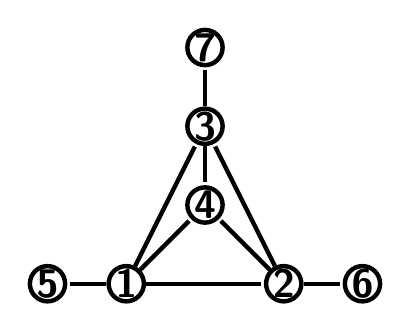
\begin{tikzpicture}[shorten >=1pt, auto, node distance=3cm, ultra thick,main node/.style={circle,draw,minimum size=.4cm,inner sep=0pt]}]%fill=black,
\begin{scope}[every node/.style={font=\sffamily\Large\bfseries}]
\node[main node] (v1) at (1,0) {1};
\node[main node] (v2) at (3,0) {2};
\node[main node] (v3) at (2,2) {3};
\node[main node] (v4) at (2,1) {4};
\node[main node] (v5) at (0,0) {5};
\node[main node] (v6) at (4,0) {6};
\node[main node] (v7) at (2,3) {7};
%\node[main node] (v) at (,) {};
\end{scope}
\begin{scope}
\draw  (v1) edge node{} (v2);
\draw  (v1) edge node{} (v3);
\draw  (v1) edge node{} (v4);
\draw  (v1) edge node{} (v5);
\draw  (v2) edge node{} (v3);
\draw  (v2) edge node{} (v4);
\draw  (v2) edge node{} (v6);
\draw  (v3) edge node{} (v4);
\draw  (v3) edge node{} (v7);
%\draw  (v) edge node{} (v);
\end{scope}
\end{tikzpicture}
\caption*{Graf $G$ który zawiera $K_4$ jako minor}
\end{figure}
\end{minipage}
\begin{minipage}{.32\textwidth}
\begin{figure}[H]
\centering
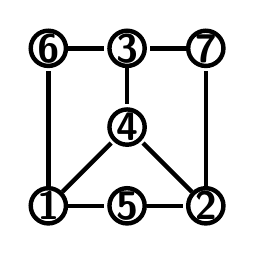
\begin{tikzpicture}[shorten >=1pt, auto, node distance=3cm, ultra thick,main node/.style={circle,draw,minimum size=.4cm,inner sep=0pt]}]%fill=black,
\begin{scope}[every node/.style={font=\sffamily\Large\bfseries}]
\node[main node] (v1) at (0,0) {1};
\node[main node] (v2) at (2,0) {2};
\node[main node] (v3) at (1,2) {3};
\node[main node] (v4) at (1,1) {4};
\node[main node] (v5) at (1,0) {5};
\node[main node] (v6) at (0,2) {6};
\node[main node] (v7) at (2,2) {7};
%\node[main node] (v) at (,) {};
\end{scope}
\begin{scope}
\draw  (v1) edge node{} (v5);
\draw  (v1) edge node{} (v6);
\draw  (v1) edge node{} (v4);
\draw  (v2) edge node{} (v7);
\draw  (v2) edge node{} (v4);
\draw  (v3) edge node{} (v4);
\draw  (v5) edge node{} (v2);
\draw  (v6) edge node{} (v3);
\draw  (v7) edge node{} (v3);
%\draw  (v) edge node{} (v);
\end{scope}
\end{tikzpicture}
\caption*{Graf $G$ zawiera topologiczną kopię $K_4$}
\end{figure}
\end{minipage}


\paragraph{A3} Zbadaj planarność poniższych grafów. Jeśli graf jest planarny, to narysuj go płasko, czyli tak, by żadne dwie krawędzie nie miały punktów wspólnych (z wyjątkiem końców). Jeżeli graf nie jest planarny, to:
\begin{itemize}
\item znajdź w nim topologiczną kopię jednego z grafów $K_{3,3}$ lub $K_5$,
\item wskaż w nim odpowiedni podział wierzchołków, świadczący o tym, że graf zawiera $K_{3,3}$ lub $K_5$ jako minor.
\end{itemize}
\begin{enumerate}[label=\alph*)]
\begin{minipage}{.25\textwidth}
\item 3-kostka
\end{minipage}
\begin{minipage}{.25\textwidth}
\item 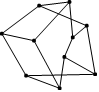
\includegraphics{img/g4}
\end{minipage}
\begin{minipage}{.25\textwidth}
\item 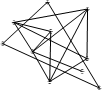
\includegraphics{img/g5}
\end{minipage}
\begin{minipage}{.25\textwidth}
\item 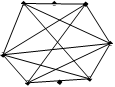
\includegraphics{img/g6}
\end{minipage}
\begin{minipage}{.25\textwidth}
\item 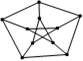
\includegraphics{img/g7}
\end{minipage}
\end{enumerate}

\textbf{Odpowiedź:}
\begin{enumerate}[label=\alph*)]
\item %Hańba mi za CtrlC CtrlV
{
%ŚCIĄGA: http://tex.stackexchange.com/questions/29246/factorial-design-diagrams-in-tikz
\newcommand\drawplane[2]
{%
    \draw
    [
        thick,
        opacity=.6,
        draw=#2,
        fill=#2!60,
    ] #1 -- cycle;%
}

\newcommand\drawonecase[4]
{
    \begin{tikzpicture}[scale=2]

        \tikzset
        {
            edgevis/.style={black},
            edgehid/.style={dashed,black},
        }

        \def\vertexradius{.7pt}

        \coordinate (OOO) at (0,0);
        \coordinate (OOI) at (xyz cs:z=1);
        \coordinate (OIO) at (xyz cs:y=1);
        \coordinate (OII) at (xyz cs:y=1,z=1);
        \coordinate (IOO) at (xyz cs:x=1);
        \coordinate (IOI) at (xyz cs:x=1,z=1);
        \coordinate (IIO) at (xyz cs:x=1,y=1);
        \coordinate (III) at (xyz cs:x=1,y=1,z=1);

        \drawplane{#1}{#2}
        \drawplane{#3}{#4}

        \draw[edgevis] (OOI) -- (OII) -- (OIO) -- (IIO) -- (IOO) -- (IOI) -- cycle;
        \draw[edgevis] (III) -- (IIO);
        \draw[edgevis] (III) -- (IOI);
        \draw[edgevis] (III) -- (OII);
        \draw[edgehid] (OOO) -- (OOI);
        \draw[edgehid] (OOO) -- (OIO);
        \draw[edgehid] (OOO) -- (IOO);

        \draw (OOO) circle (\vertexradius);
        \draw (OOI) circle (\vertexradius);
        \draw (OIO) circle (\vertexradius);
        \draw (OII) circle (\vertexradius);
        \draw (IOO) circle (\vertexradius);
        \draw (IOI) circle (\vertexradius);
        \draw (IIO) circle (\vertexradius);
        \draw (III) circle (\vertexradius);

    \end{tikzpicture}
}
$Q_4$:
\begin{minipage}{.48\textwidth}
\begin{figure}[H]
\centering
\drawonecase
                {(OOO) -- (OOI) -- (OII) -- (OIO)}{red}
                {(IOO) -- (IOI) -- (III) -- (IIO)}{blue}
\end{figure}
\end{minipage}
\begin{minipage}{.48\textwidth}
\begin{figure}[H]
\centering
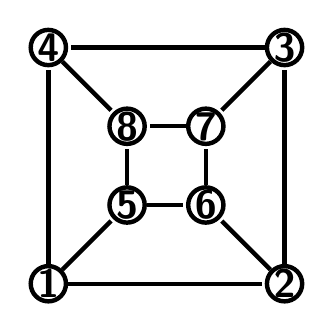
\begin{tikzpicture}[shorten >=1pt, auto, node distance=3cm, ultra thick,main node/.style={circle,draw,minimum size=.4cm,inner sep=0pt]}]%fill=black,
\begin{scope}[every node/.style={font=\sffamily\Large\bfseries}]
\node[main node] (v1) at (0,0) {1};
\node[main node] (v2) at (3,0) {2};
\node[main node] (v3) at (3,3) {3};
\node[main node] (v4) at (0,3) {4};
\node[main node] (v5) at (1,1) {5};
\node[main node] (v6) at (2,1) {6};
\node[main node] (v7) at (2,2) {7};
\node[main node] (v8) at (1,2) {8};
%\node[main node] (v) at (,) {};
\end{scope}
\begin{scope}
\draw  (v1) edge node{} (v2);
\draw  (v1) edge node{} (v4);
\draw  (v1) edge node{} (v5);
\draw  (v2) edge node{} (v3);
\draw  (v2) edge node{} (v6);
\draw  (v3) edge node{} (v4);
\draw  (v3) edge node{} (v7);
\draw  (v4) edge node{} (v8);
\draw  (v5) edge node{} (v6);
\draw  (v5) edge node{} (v8);
\draw  (v6) edge node{} (v7);
\draw  (v7) edge node{} (v8);
%\draw  (v) edge node{} (v);
\end{scope}
\end{tikzpicture}
\end{figure}
\end{minipage}
}
\item 
\begin{minipage}{.48\textwidth}
\begin{figure}[H]
\centering
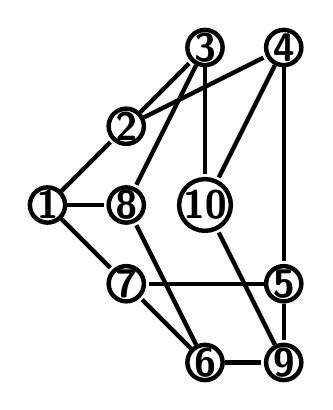
\begin{tikzpicture}[shorten >=1pt, auto, node distance=3cm, ultra thick,main node/.style={circle,draw,minimum size=.4cm,inner sep=0pt]}]%fill=black,
\begin{scope}[every node/.style={font=\sffamily\Large\bfseries}]
\node[main node] (v1) at (0,0) {1};
\node[main node] (v2) at (1,1) {2};
\node[main node] (v3) at (2,2) {3};
\node[main node] (v4) at (3,2) {4};
\node[main node] (v5) at (3,-1) {5};
\node[main node] (v6) at (2,-2) {6};
\node[main node] (v7) at (1,-1) {7};
\node[main node] (v8) at (1,0) {8};
\node[main node] (v9) at (3,-2) {9};
\node[main node] (v10) at (2,0) {10};
%\node[main node] (v) at (,) {};
\end{scope}
\begin{scope}
\draw  (v1) edge node{} (v2);
\draw  (v1) edge node{} (v7);
\draw  (v1) edge node{} (v8);
\draw  (v2) edge node{} (v3);
\draw  (v2) edge node{} (v4);
\draw  (v3) edge node{} (v8);
\draw  (v3) edge node{} (v10);
\draw  (v4) edge node{} (v5);
\draw  (v4) edge node{} (v10);
\draw  (v5) edge node{} (v7);
\draw  (v5) edge node{} (v9);
\draw  (v6) edge node{} (v7);
\draw  (v6) edge node{} (v8);
\draw  (v6) edge node{} (v9);
\draw  (v9) edge node{} (v10);
%\draw  (v) edge node{} (v);
\end{scope}
\end{tikzpicture}
\caption*{Oryginalny rysunek}
\end{figure}
\end{minipage}
\begin{minipage}{.48\textwidth}
\begin{figure}[H]
\centering
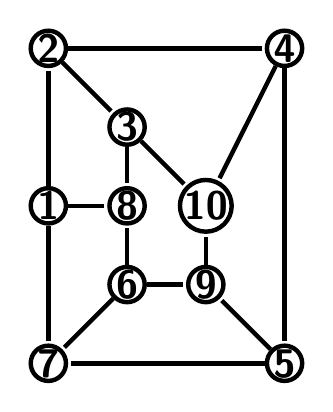
\begin{tikzpicture}[shorten >=1pt, auto, node distance=3cm, ultra thick,main node/.style={circle,draw,minimum size=.4cm,inner sep=0pt]}]%fill=black,
\begin{scope}[every node/.style={font=\sffamily\Large\bfseries}]
\node[main node] (v1) at (0,0) {1};
\node[main node] (v2) at (0,2) {2};
\node[main node] (v3) at (1,1) {3};
\node[main node] (v4) at (3,2) {4};
\node[main node] (v5) at (3,-2) {5};
\node[main node] (v6) at (1,-1) {6};
\node[main node] (v7) at (0,-2) {7};
\node[main node] (v8) at (1,0) {8};
\node[main node] (v9) at (2,-1) {9};
\node[main node] (v10) at (2,0) {10};
%\node[main node] (v) at (,) {};
\end{scope}
\begin{scope}
\draw  (v1) edge node{} (v2);
\draw  (v1) edge node{} (v7);
\draw  (v1) edge node{} (v8);
\draw  (v2) edge node{} (v3);
\draw  (v2) edge node{} (v4);
\draw  (v3) edge node{} (v8);
\draw  (v3) edge node{} (v10);
\draw  (v4) edge node{} (v5);
\draw  (v4) edge node{} (v10);
\draw  (v5) edge node{} (v7);
\draw  (v5) edge node{} (v9);
\draw  (v6) edge node{} (v7);
\draw  (v6) edge node{} (v8);
\draw  (v6) edge node{} (v9);
\draw  (v9) edge node{} (v10);
%\draw  (v) edge node{} (v);
\end{scope}
\end{tikzpicture}
\caption*{Ctrl C Ctrl V ze zmianą położenia wierzchołków}
\end{figure}
\end{minipage}

\item Pewnie tego nie widać, ale podany graf zawiera dwie składowe - nie jest spójny - trójkąt i to drugie, ogólnie obydwie części są planarne, więc graf jest planarny.\\
\begin{minipage}{.45\textwidth}
\begin{figure}[H]
\centering
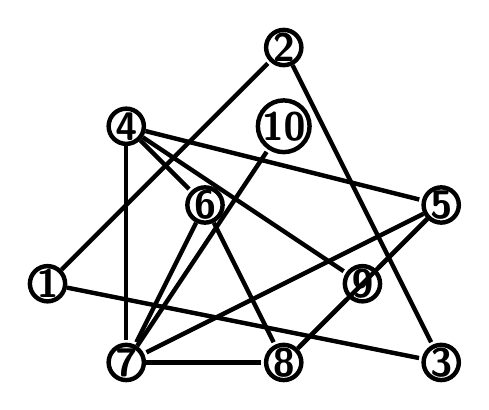
\begin{tikzpicture}[shorten >=1pt, auto, node distance=3cm, ultra thick,main node/.style={circle,draw,minimum size=.4cm,inner sep=0pt]}]%fill=black,
\begin{scope}[every node/.style={font=\sffamily\Large\bfseries}]
\node[main node] (v1) at (-1,0) {1};
\node[main node] (v2) at (2,3) {2};
\node[main node] (v3) at (4,-1) {3};
\node[main node] (v4) at (0,2) {4};
\node[main node] (v5) at (4,1) {5};
\node[main node] (v6) at (1,1) {6};
\node[main node] (v7) at (0,-1) {7};
\node[main node] (v8) at (2,-1) {8};
\node[main node] (v9) at (3,0) {9};
\node[main node] (v10) at (2,2) {10};
%\node[main node] (v) at (,) {};
\end{scope}
\begin{scope}
\draw  (v1) edge node{} (v2);
\draw  (v1) edge node{} (v3);
\draw  (v2) edge node{} (v3);
\draw  (v4) edge node{} (v5);
\draw  (v4) edge node{} (v6);
\draw  (v4) edge node{} (v7);
\draw  (v4) edge node{} (v9);
\draw  (v5) edge node{} (v7);
\draw  (v5) edge node{} (v8);
\draw  (v5) edge node{} (v9);
\draw  (v6) edge node{} (v7);
\draw  (v6) edge node{} (v8);
\draw  (v7) edge node{} (v8);
\draw  (v7) edge node{} (v10);
\draw  (v8) edge node{} (v9);
%\draw  (v) edge node{} (v);
\end{scope}
\end{tikzpicture}
\caption*{}
\end{figure}
\end{minipage}
\begin{minipage}{.45\textwidth}
\begin{figure}[H]
\centering
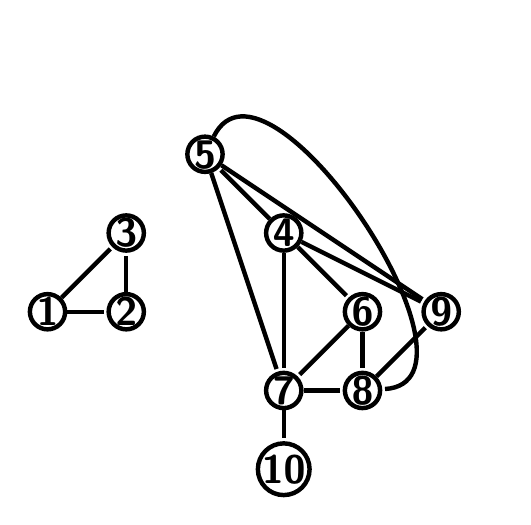
\begin{tikzpicture}[shorten >=1pt, auto, node distance=3cm, ultra thick,main node/.style={circle,draw,minimum size=.4cm,inner sep=0pt]}]%fill=black,
\begin{scope}[every node/.style={font=\sffamily\Large\bfseries}]
\node[main node] (v1) at (0,0) {1};
\node[main node] (v2) at (1,0) {2};
\node[main node] (v3) at (1,1) {3};
\node[main node] (v4) at (3,1) {4};
\node[main node] (v5) at (2,2) {5};
\node[main node] (v6) at (4,0) {6};
\node[main node] (v7) at (3,-1) {7};
\node[main node] (v8) at (4,-1) {8};
\node[main node] (v9) at (5,0) {9};
\node[main node] (v10) at (3,-2) {10};
%\node[main node] (v) at (,) {};
\end{scope}
\begin{scope}
\draw  (v1) edge node{} (v2);
\draw  (v1) edge node{} (v3);
\draw  (v2) edge node{} (v3);
\draw  (v4) edge node{} (v5);
\draw  (v4) edge node{} (v6);
\draw  (v4) edge node{} (v7);
\draw  (v4) edge node{} (v9);
\draw  (v5) edge node{} (v7);
\draw[bend left=120]  (v5) edge node{} (v8);
\draw  (v5) edge node{} (v9);
\draw  (v6) edge node{} (v7);
\draw  (v6) edge node{} (v8);
\draw  (v7) edge node{} (v8);
\draw  (v7) edge node{} (v10);
\draw  (v8) edge node{} (v9);
%\draw  (v) edge node{} (v);
\end{scope}
\end{tikzpicture}
\caption*{Jak się to ładnie narysuje to jest git}
\end{figure}
\end{minipage}

\item 
\begin{minipage}{.45\textwidth}
\begin{figure}[H]
\centering
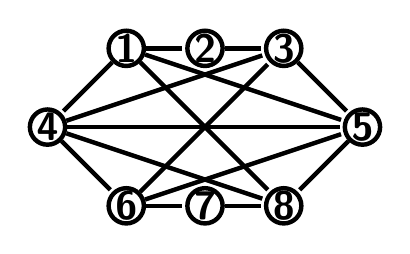
\begin{tikzpicture}[shorten >=1pt, auto, node distance=3cm, ultra thick,main node/.style={circle,draw,minimum size=.4cm,inner sep=0pt]}]%fill=black,
\begin{scope}[every node/.style={font=\sffamily\Large\bfseries}]
\node[main node] (v1) at (0,2) {1};
\node[main node] (v2) at (1,2) {2};
\node[main node] (v3) at (2,2) {3};
\node[main node] (v4) at (-1,1) {4};
\node[main node] (v5) at (3,1) {5};
\node[main node] (v6) at (0,0) {6};
\node[main node] (v7) at (1,0) {7};
\node[main node] (v8) at (2,0) {8};
%\node[main node] (v) at (,) {};
\end{scope}
\begin{scope}
\draw  (v1) edge node{} (v2);
\draw  (v1) edge node{} (v4);
\draw  (v1) edge node{} (v5);
\draw  (v1) edge node{} (v8);
\draw  (v4) edge node{} (v3);
\draw  (v4) edge node{} (v5);
\draw  (v4) edge node{} (v6);
\draw  (v4) edge node{} (v8);
\draw  (v6) edge node{} (v3);
\draw  (v6) edge node{} (v5);
\draw  (v6) edge node{} (v7);
\draw  (v2) edge node{} (v3);
\draw  (v3) edge node{} (v5);
\draw  (v5) edge node{} (v8);
\draw  (v7) edge node{} (v8);
%\draw  (v) edge node{} (v);
\end{scope}
\end{tikzpicture}
\caption*{Ogryginalny graf.}
\end{figure}
\end{minipage}
\begin{minipage}{.45\textwidth}
\begin{figure}[H]
\centering
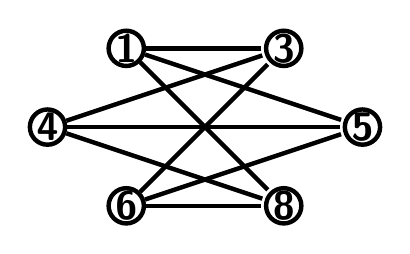
\begin{tikzpicture}[shorten >=1pt, auto, node distance=3cm, ultra thick,main node/.style={circle,draw,minimum size=.4cm,inner sep=0pt]}]%fill=black,
\begin{scope}[every node/.style={font=\sffamily\Large\bfseries}]
\node[main node] (v1) at (0,2) {1};
\node[main node] (v3) at (2,2) {3};
\node[main node] (v4) at (-1,1) {4};
\node[main node] (v5) at (3,1) {5};
\node[main node] (v6) at (0,0) {6};
\node[main node] (v8) at (2,0) {8};
%\node[main node] (v) at (,) {};
\end{scope}
\begin{scope}
\draw  (v1) edge node{} (v3);
\draw  (v1) edge node{} (v5);
\draw  (v1) edge node{} (v8);
\draw  (v4) edge node{} (v3);
\draw  (v4) edge node{} (v5);
\draw  (v4) edge node{} (v8);
\draw  (v6) edge node{} (v3);
\draw  (v6) edge node{} (v5);
\draw  (v6) edge node{} (v8);
%\draw  (v) edge node{} (v);
\end{scope}
\end{tikzpicture}
\caption*{Minor grafu $K_{3,3}$ usunięcie wierzchołków: $\{2, 7\}$, usunięcie krawędzi krawędzi:  $\{1,4\},\{4,6\},\{3,5\},\{5,8\}$.} 
\end{figure}
\end{minipage}

\item Ogólne to graf Petersena - nie plenarny (ale fajny do narysowania) można z niego zrobić $K_5$
\begin{figure}[H]
\centering
\begin{tikzpicture}[every node/.style={draw,circle,very thick}]
  \graph[clockwise, radius=2cm] {subgraph C_n [n=5,name=A] };
  \graph[clockwise, radius=1cm] {subgraph I_n [n=5,name=B] };

  \foreach \i [evaluate={\j=int(mod(\i+2+4,5)+1)}]% using Paul Gaborit's optimisation
     in {1,2,3,4,5}{
    \draw (A \i) -- (B \i);
    \draw (B \j) -- (B \i);
  }
\end{tikzpicture}
\end{figure}


\end{enumerate}

\paragraph{A4}
\begin{enumerate}[label=\alph*)]
\item Czy pełny graf dwudzielny $K_{3,3}$ zawiera jako minor graf $K_4$ ?
\item Czy pełny graf dwudzielny $K_{8,4}$ zawiera jako minor graf $K_5$ ?
\end{enumerate}
\textbf{Odpowiedź:} 
\begin{enumerate}[label=\alph*)]
\item TAK, DA SIĘ
\item TAK, DA SIĘ
\end{enumerate}

\paragraph{A5} Czy istnieje graf planarny $G$, dla którego
\begin{enumerate}[label=\alph*)]
\item  $V(G) = 7$ i $E(G) = 15$?
\item  $V(G) = 7$ i $E(G) = 17$?
  \item  $\delta (G) = 6$?
\end{enumerate}
Jeżeli istnieje, to narysuj przykład.

\textbf{Odpowiedź:} 
\todo[inline,color=red]{dowód nie wprost}
\begin{enumerate}[label=\alph*)]
\item Zgodnie z twierdzeniem, ze jeżeli graf $G=(V,E)$ jest spójny, prosty i planarny to prawdziwy jes wzór:
$$E(G)\leq 3*V(G)-6$$
to dla wartości: $E(G)=15$ i $V(G)=7$ otrzymujemy, że $15\leq 15$
\begin{figure}[H]
\centering
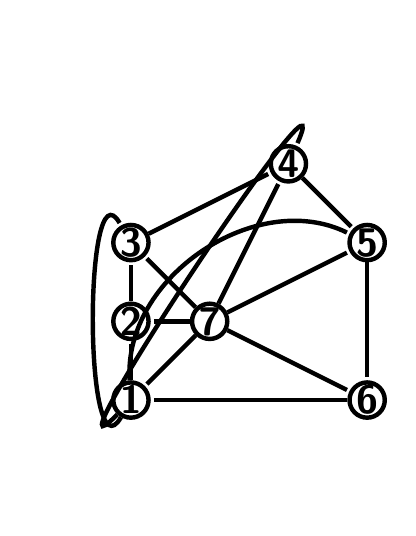
\begin{tikzpicture}[shorten >=1pt, auto, node distance=3cm, ultra thick,main node/.style={circle,draw,minimum size=.4cm,inner sep=0pt]}]%fill=black,
\begin{scope}[every node/.style={font=\sffamily\Large\bfseries}]
\node[main node] (v1) at (0,0) {1};
\node[main node] (v2) at (0,1) {2};
\node[main node] (v3) at (0,2) {3};
\node[main node] (v4) at (2,3) {4};
\node[main node] (v5) at (3,2) {5};
\node[main node] (v6) at (3,0) {6};
\node[main node] (v7) at (1,1) {7};
%\node[main node] (v) at (,) {};
\end{scope}
\begin{scope}
\draw  (v1) edge node{} (v2);
\draw  (v2) edge node{} (v3);
\draw  (v3) edge node{} (v4);
\draw  (v4) edge node{} (v5);
\draw  (v5) edge node{} (v6);
\draw  (v6) edge node{} (v1);
\draw  (v7) edge node{} (v1);
\draw  (v7) edge node{} (v2);
\draw  (v7) edge node{} (v3);
\draw  (v7) edge node{} (v4);
\draw  (v7) edge node{} (v5);
\draw  (v7) edge node{} (v6);
\draw[bend left=150]  (v1) edge node{} (v3);
\draw[bend left=170]  (v1) edge node{} (v4);
\draw[bend right=300]  (v1) edge node{} (v5);
%\draw  (v) edge node{} (v);
\end{scope}
\end{tikzpicture}
\caption*{Jak się to łanie narysuje, to żadna krawędź na siebie nie nachodzi.}
\end{figure}

\item Nie spełnia wyżej wymienionego twierdzenia, albowiem: $17\not \leq 15$. \\
Nie wiem czy tak mogę, ale jeżeli graf $G=(V,E)$ jest spójny, prosty i planarny to spełnia równanie, dowód nie wprost?
\todo[inline,color=purple]{Czy to działa w drugą stronę?}

\item jeżeli $\delta (G) = 6$ to w mamy przynajmniej graf $K_7$ który zawiera topologiczną kopię $K_5$ przez co nie spełnia twierdzenie Kuratowskiego (\ref{the:Kuratowski} na stronie \pageref{the:Kuratowski}).
\end{enumerate}


\paragraph{A6} Wyznacz liczbę chromatyczną obu grafów nr (7) narysowanych na końcu listy ,,Rozgrzewka grafowa''.

\textbf{Odpowiedź:} 
\begin{enumerate}[label=\alph*)]
\item 3
\item 3
\end{enumerate}
jeżeli chodzi o te kółka-grafy

cykl na 3 wierzchołkach można zrobić na 3 kolorach



\paragraph{A7} Graf $G$ otrzymany jest z grafu pełnego $K_{20}$ na $20$ wierzchołkach przez usunięcie z niego krawędzi czterech wierzchołkowo rozłącznych trójkątów (tzn. $K_3$). Znajdź liczbę chromatyczną grafu $G$.

\todo[inline,color=orange]{Przerysować rysunek!}
$\chi \leq 12$

\paragraph{A8} Załóżmy, że graf $G$ jest niespójny i znamy liczbę chromatyczną każdej jego składowej. Ile wynosi $\chi (G)$?
Rozwiąż to zadanie, nie korzystając z żadnych twierdzeń.

\textbf{Odpowiedź:} 
Graf $G$ jest niespójny $\rightarrow $ zawiera 2 lub więcej składowych ($G_i$) i znamy liczbę chromatyczną każdej składowej: $\chi (G_i)$.

$$\chi (G) = \left\{\forall _{G_i \subset G} \max (\chi (G_i)) \right\}$$
Maksymalna liczba chromatyczna ,,podgrafu'' będzie determinowała liczbę chromatyczną całego grafu.
\todo[inline,color=brown]{DOWÓD!}

\paragraph{A9} Oceń poprawność każdego z poniższych zdań. W każdym przypadku poprzyj odpowiedź, w zależności od potrzeby, uzasadnieniem ogólnym, przykładem lub kontrprzykładem. Uwaga: Tu i w innych zadaniach
graf o liczbie chromatycznej co najwyżej $k$ nazywamy grafem $k-$ kolorowanym.
\begin{enumerate}[label=\alph*)]
\item Jeśli $E(G) < 3V(G) - 6$, to $G$ jest planarny.
\\\textbf{Odpowiedź:} \\
Twierdzenie odwrotne do Eulera $\Rightarrow$ NIE DZIAŁA 
\begin{figure}[H]
\centering
\begin{tikzpicture}[every node/.style={draw,circle,very thick}]
  \graph[clockwise, radius=2cm] {subgraph C_n [n=5,name=A] };
  \graph[clockwise, radius=1cm] {subgraph I_n [n=5,name=B] };

  \foreach \i [evaluate={\j=int(mod(\i+2+4,5)+1)}]% using Paul Gaborit's optimisation
     in {1,2,3,4,5}{
    \draw (A \i) -- (B \i);
    \draw (B \j) -- (B \i);
  }
\end{tikzpicture}
\caption*{Ten fajny graf Petersena}
\end{figure}
$V(G)=10,\ E(G)=15$ i przedstawiony wzór jest spełniony a to nie jest graf planarny!

\item Jeżeli graf nie zawiera ani $K_5$ , ani $K_{3,3}$ , to jest planarny.
\\\textbf{Odpowiedź:} \\
$G \not \triangleright K_5 \land G \not \triangleright K_{3,3} \Rightarrow G $ jest planarny\\
NIE przykład d z A3

\item Jeśli $E(G) > 3V(G) - 6$, to graf $G$ nie jest planarny.
\\\textbf{Odpowiedź:} \\
NIET *--*

\item Jeśli $E(G) > 3V(G) - 6$ i $V(G) < 3$, to graf $G$ jest planarny.
\\\textbf{Odpowiedź:} \\ TAK

\item Dla ustalonego spójnego grafu planarnego każdy jego płaski rysunek ma tyle samo ścian.
\\\textbf{Odpowiedź:} \\  TAK

\item Jeżeli graf jest 4-kolorowalny, to jest planarny.
\\\textbf{Odpowiedź:} \\ NIE graf Petersona 

\item Jeżeli graf jest planarny, to jest 4-kolorowalny.
\\\textbf{Odpowiedź:} \\ TAK twierdzenie o 4 kolorach

\item Z wzoru Eulera wynika, że nie istnieje graf płaski (czyli płasko narysowany grafu planarny), który ma dokładnie $6$ wierzchołków, $6$ krawędzi i $3$ ściany.
\\\textbf{Odpowiedź:} \\ NIE

\item Każdy graf dwudzielny jest 2-kolorowalny.
\\\textbf{Odpowiedź:} \\ TAK

\item Każdy graf dwudzielny ma liczbę chromatyczną $2$.
\\\textbf{Odpowiedź:} \\ jeden wierzchołek

\item Żaden graf 2-kolorowalny nie zawiera $K_3$ .
\\\textbf{Odpowiedź:} \\ $K_3$ tak dowód nie wprost

\item Jeżeli graf nie zawiera $K_3$ , to jest 2-kolorowalny.
\\\textbf{Odpowiedź:} \\ nie kontrprzykład

\item Liczba chromatyczna cyklu nieparzystego wynosi $3$.
\\\textbf{Odpowiedź:} \\ TAK dowód nie wprost, 3 da się.

\end{enumerate}

\subsection{Zadania Domowe B}
\paragraph{B1} Wyznacz wszystkie k, dla których k–kostka jest grafem planarnym.

\paragraph{B2} Uzasadnij, nie Korzystając ani z twierdzenia Kuratowskiego, ani z twierdzenia Wagnera, że wszystkie
grafy dwudzielne na 6 wierzchołkach, prócz $K_{3,3}$, są planarne.

\paragraph{B3} Czy istnieje graf planarny $G$, dla którego
\begin{enumerate}[label=\alph*)]
\item $V(G) = 100$ i $E(G) = 296$?
\item $V(G) = 100$ i $E(G) = 190$?
\end{enumerate}

\paragraph{B4} Na płaszczyźnie znajduje się skończony (i niepusty) zbiór punktów, przy czym między każdą
parą punktów odległość jest nie mniejsza niż 1. każdą parę punktów będących w odległości dokładnie 1 połączono odcinkiem.
\begin{enumerate}[label=\alph*)]
\item Czy tak powstały graf jest planarny?
\item Jakich wartości na pewno nie przyjmie liczba chromatyczna takiego grafu?
\item Jakie wartości może przyjąć liczba chromatyczna takiego grafu? Wyznacz tyle możliwości, ile potrafisz (im więcej tym lepiej). Najlepiej znaleźć wszystkie i udowodni, że nie ma innych.
\end{enumerate}

\paragraph{B5}
\begin{enumerate}[label=\alph*)]
\item Ile ścian ma triangulacja na n wierzchołkach?
\item Ile wierzchołków ma triangulacja o 100 ścianach?
\item Czy dla każdego $s > 100$ istnieje triangulacja o s ścianach?
\item Załóżmy, że pewna triangulacja ma 496 ścian. Ile ma wierzchołków?
\item Czy dopełnienie triangulacji może być grafem, którego płaski rysunek jest triangulacją? 
\end{enumerate}

\paragraph{B6} Firma komputerowa Myrdyrda postanowiła nagrodzić 12 swoich najwierniejszych klientw zapraszając
ich na szkolenie dotyczące ich ulubionych aplikacji. każdy ze szczęśliwej dwunastki mógł wybrać 3 spośród dostępnych 59 aplikacji firmy Myrdyrda, a firma gwarantuje jednodniowe kursy poświęcone każdej aplikacji
z wybranej trójki. Kierownik firmy chce zaplanować kursy tak, by szkolenie trwało jak najkrócej.
\begin{enumerate}[label=\alph*)]
\item Jaki problem grafowy musi on rozwiązać?
\item Czy prawdą jest, że bez względu na wybór aplikacji przez uczestników, kursy można zaplanować w ten sposób, by szkolenie trwało nie dłużej niż 5 dni?
\end{enumerate}
Przypomnijmy raz jeszcze zasady:
\begin{itemize}
\item każdy z dwanaściorga uczestników powinien wziąć udział w trzech kursach poświęconych wybranym przez siebie aplikacjom.
\item każdy z uczestników może wziąć udział w co najwyżej jednym kursie dziennie.
\item każdy z kursów odbywa się w czasie szkolenia dokładnie raz.
\end{itemize}

\paragraph{B7} W jaki sposób pokolorować w sposób właściwy wierzchołki
\begin{enumerate}[label=\alph*)]
\item dowolnej ścieżki, mając dwa kolory?
\item dowolnego drzewa, mając dwa kolory?
\item dowolnego grafu, którego maksymalny stopień wynosi 3, mając cztery kolory?
Opisz ideę algorytmu.
\end{enumerate}

\paragraph{B8} Wyznacz liczbę chromatyczną:
\begin{enumerate}[label=\alph*)]
\item każdego niepustego drzewa,
\item kraty $5 \times 5$,
\item  kraty $5 \times 5$, w której połączono krawędzią lewy dolny wierzchołek z prawym górnym wierzchołkiem, a prawy dolny – z wierzchołkiem lewym górnym.
\item  grafu $G$ o 20 wierzchołkach, otrzymanego z grafu pełnego $K_{20}$ na 20 wierzchołkach przez usunięcie z
niego krawędzi czterech wierzchołkowo rozłącznych trójkątów.
\end{enumerate}

\paragraph{B9} Uzasadnij (nie Korzystając z żadnych twierdzeń), że
\begin{enumerate}[label=\alph*)]
\item Jeżeli graf jest 2-kolorowalny, to nie zawiera nieparzystych cykli.
\item Jeżeli graf nie zawiera nieparzystych cykli, to jest 2-kolorowalny.
\end{enumerate}

\paragraph{B10} Jaka jest najmniejszą możliwa, a jaka największa możliwa liczba chromatyczna grafu 5-regularnego?

\paragraph{B11} Załóżmy, że liczba chromatyczna pewnego grafu o 17 wierzchołkach jest mniejsza niż 4. Uzasadnij, że w grafie tym zawsze znajdziemy sześć wierzchołków, między którymi nie ma żadnych krawędzi.

\paragraph{B12} oceń poprawność każdego z poniższych zdań. W każdym przypadku poprzyj odpowiedź, w zależności od potrzeb, uzasadnieniem ogólnym, przykładem lub kontrprzykładem.
\begin{enumerate}[label=\alph*)]
\item Jeśli graf zawiera topologiczną kopię grafu $K_5$, to zawiera jako minor graf $K_5$.
\item Jeśli graf zawiera jako minor grafu $K_5$, to zawiera topologiczną kopię grafu $K_5$.
\item Jeśli graf zawiera $K_{3,3}$ jako minor lub $K_5$ jako minor, to zawiera topologiczną kopię grafu $K_{3,3}$ lub topologiczną kopię grafu $K_5$.
\item Jeśli graf $G$ zawiera $K_5$ jako minor, to $\chi (G) > 5$.
\item Istnieje graf $G$, dla którego $\chi (G) > 4$, a który nie zawiera $K_4$.
\item Nie istnieje Spójny graf płaski (czyli p lasko narysowany grafu planarny), który ma dokładnie 100 wierzchołków, 150 krawędzi i 50 ścian.
\item dopełnienie spójnego grafu płaskiego o 20 wierzchołkach i 30 ścianach ma 142 krawędzie.
\item Twierdzenie odwrotne do twierdzenia o czterech kolorach jest prawdziwe.
\item Istnieje graf planarny o przynajmniej 11 wierzchołkach, którego dopełnienie jest grafem planarnym.
\item Istnieje graf G, innych niż cykl nieparzysty lub graf pełny, dla którego $\chi (G) = \Delta (G) + 1$.
\item Istnieje graf 4-regularny G na 10 wierzchołkach, dla którego $\chi (G) = 5$.
\end{enumerate}


\subsection{Zadania}
\paragraph{Zad.1} Uzasadnij, nie Korzystając ani z twierdzenia Kuratowskiego, ani z twierdzenia Wagnera, że wszystkie grafy na 5 wierzchołkach, oprócz K5, są planarne.

\paragraph{Zad.2} Wyprowadź odpowiednik wzoru Eulera dla grafu płaskiego o t składowych.

\paragraph{Zad.3} Czy istnieje graf planarny G, dla którego v(G) = 100 i e(G) = 294 ?

\paragraph{Zad.4} Ile krawędzi ma triangulacja o n > 3 wierzchołkach?

\paragraph{Zad.5} Graf G o 212 wierzchołkach jest dopełnieniem grafu składającego się z 154 składowych, z których 4 to cykle o długości trzy, 50 to izolowane krawędzie, a pozostałe 100 to wierzchołki izolowane. Znajdź liczbę chromatyczną grafu G.

\paragraph{Zad.6} Podaj interpretację grafową następującego problemu. Jakiego parametru grafowego tu szukamy?
Układamy plan sesji egzaminacyjnej tak, by każdy student miał co najwyżej jeden egzamin w ciągu dnia. Chcemy znaleźć najmniejszą możliwą liczbę dni potrzebną na zaplanowanie wszystkich egzaminów.

\paragraph{Zad.7} W jaki sposób pokolorować w sposób właściwy
\begin{enumerate}[label=\alph*)]
\item wierzchołki grafu, którego maksymalny stopień wynosi $\Delta $, mając $\Delta +1$ kolorów?
\item wierzchołki grafu planarnego, mając 6 kolorów?

\textbf{Odpowiedź: }kolorowanie srosu
\end{enumerate}
